\documentclass{sig-alternate}

\begin{document}

\title{Simulando una cola simple}

\numberofauthors{2}

\author{
    \alignauthor
    Sessa, Carlos\\
    \email{csessa@alu.itba.edu.ar} \\
    \ \\
    Abramowicz, Pablo\\
    \email{pabramow@alu.itba.edu.ar} \\
    \ \\
    \alignauthor
    Gomez Vidal, Maximiliano\\
    \email{dgomezvi@alu.itba.edu.ar} \\
    \ \\
    Villa Fern\'{a}ndez, Santiago\\
    \email{svillafe@alu.itba.edu.ar}
}

\maketitle

\begin{abstract}
En este art\'{i}culo se simula un sistema de cola simple y se estiman
par\'{a}metros tales como la longitud media de la cola y el tiempo de
atenci\'{o}n. Se analiza tambi\'{e}n el costo operativo asociado.
\end{abstract}

\keywords{Modelo de cola simple, FIFO, tiempo de espera, sistema de atenci\'{o}n
al cliente, servidor simple}

\section{Introducci\'{o}n}\label{introduccion}

Las colas se utilizan en diversos \'{a}mbitos, tales como sistemas 
inform\'{a}ticos, transportes y operaciones de investigaci\'{o}n, entre otros. 
Los objetos, personas o eventos son tomados 
como datos que se almacenan para su posterior procesamiento.


La cola simple, denominada $M/M/1/\infty/FIFO$ o simplemente $M/M/1$, es el 
sistema m\'{a}s sencillo de analizar mediante una simulaci\'{o}n por eventos 
discretos.


El sistema de cola simple se encuentra caracterizado principalmente por el 
tiempo necesario para atender a un cliente y la tasa de llegada de los mismos.


En la secci\'{o}n \ref{modelo} se describe el modelo de cola simple y los
par\'{a}metros involucrados. En la secci\'{o}n \ref{simulacion} se realizan
las simulaciones, se estudia el comportamiento del sistema y se analiza
el costo operativo resultante. Finalmente, se exponen las conclusiones en 
la secci\'{o}n \ref{conclusiones}.

\section{Modelo de cola simple}\label{modelo}

Este modelo asume que los clientes llegan al sistema mediante un proceso de
Poisson con una tasa media de \\ $\lambda[clientes/hora]$. Tambi\'{e}n se asume
que el servidor atiende a cada uno de los clientes con un tiempo de servicio
distribuido en forma exponencial con media $1/\mu$.


Si cuando llega un nuevo cliente el servidor se encuentra libre, entonces el 
mismo es atendido en forma inmediata. Caso contrario, el cliente debe ingresar
en la cola y esperar su turno.


Resulta de inter\'{e}s poder establecer las probabilidades en estado estacionario,
cuando el sistema se encuentra en equilibrio:

\begin{equation}
\label{probabilidad_largo_plazo}
p_{n} = \lim_{t \rightarrow \infty} P \{ N_{t} = n \}
\end{equation}

donde $N_{t}$ es la cantidad de clientes en el sistema en el instante $t$.
Generalizando para el estado $n$ se obtiene una relaci\'{o}n de recurrencia
cuya soluci\'{o}n es:

\begin{equation}
\label{prob_estado_estacionario}
p_{n} = \left( \frac{\lambda}{\mu} \right)^{n} p_{0}
\end{equation}

con condiciones iniciales

\begin{equation}
\label{prob_estado_estacionario_ci}
p_{1} = \frac{\lambda}{\mu} p_{0}
\end{equation}


El factor $\rho = \lambda / \mu$ se denomina intensidad de tr\'{a}fico del
sistema. De esta forma la ecuaci\'{o}n \eqref{prob_estado_estacionario} puede
reescribirse como:

\begin{equation}
\label{prob_estado_estacionario_con_rho}
p_{n} = (1 - \rho) \rho^{n}
\end{equation}


De esta ecuaci\'{o}n se desprende que la intensidad de tr\'{a}fico debe
cumplir $\rho < 1$ para que el sistema sea estable. El caso $\rho > 1$
implica que el servidor tarda m\'{a}s tiempo en atender a un cliente que nuevos
clientes en arribar al sistema, generando as\'{i} una cola cada vez m\'{a}s 
larga.


A partir de las ecuaciones obtenidas es posible describir la longitud media
de la cola $L_{q}$ y el n\'{u}mero medio de clientes en el sistema $L$ en 
funci\'{o}n de $\rho$:

\begin{equation}
\label{longitud_media_en_la_cola}
L_{q} = \frac{\rho^{2}}{1-\rho}
\end{equation}

\begin{equation}
\label{numero_medio_clientes_en_el_sistema}
L = \frac{\rho}{1-\rho}
\end{equation}

%TODO citar a este autor
%D.C. Little
%A Proof for the Queuing Formula L = W , Operations Research, 9, 1961, pp.383­-387)

El modelo no estar\'{i}a completo sin el an\'{a}lisis del tiempo medio de 
espera, medida importante en lo que respecta a la performance del sistema
de colas. El tiempo medio de un individuo en el sistema $(W)$ y en cola $(W_{q})$
resultan:

\begin{equation}
\label{tiempo_medio_en_el_sistema}
W = \frac{1}{\mu - \lambda}
\end{equation}

\begin{equation}
\label{tiempo_medio_en_la_cola}
W_{q} = \frac{\rho}{\mu - \lambda}
\end{equation}


\section{Simulaci\'{o}n}\label{simulacion}

En primer lugar se desea estimar el promedio temporal de clientes en el sistema
y el promedio temporal de los clientes en la cola, dados por las ecuaciones:

\begin{equation}
\label{estimo_promedio_temporal_clientes_sistema}
L = \frac{1}{T} \int_{0}^{T} L(t) dt
\end{equation}

\begin{equation}
\label{estimo_promedio_temporal_clientes_cola}
L_{q} = \frac{1}{T} \int_{0}^{T} q(t) dt
\end{equation}

La cantidad de clientes en cola en el instante $t$ se encuentra representada por
la funci\'{o}n $q(t)$. $L(t)$ es la cantidad de clientes en el sistema.


Se comienza estudiando el comportamiento del sistema con una tasa de arribos
$\lambda = 1$ y un tiempo medio de servicio $1/\mu = 1.25$, ambos indicando
cantidad de clientes por hora.
La cantidad total de clientes a ser atendidos por el sistema se fija en $n=9000$.


El valor medio de clientes en cola te\'{o}rico para los par\'{a}metros
especificados resulta aproximadamente $3.2$ clientes. La estimaci\'{o}n luego
de $50$ simulaciones resulta $3.241$, presentando un error relativo del
$0.295\%$.


Resulta sumamente importante estimar tambi\'{e}n el tiempo medio que tarda
cada cliente desde que arriba al sistema hasta que termina de consumir el
servicio. 


En la figura ~\ref{fig:LvsW} se observa como var\'{i}a el tiempo medio en el sistema
$W$ a medida que la cantidad de clientes arribados aumenta.

\begin{figure*}[hp]
\centering
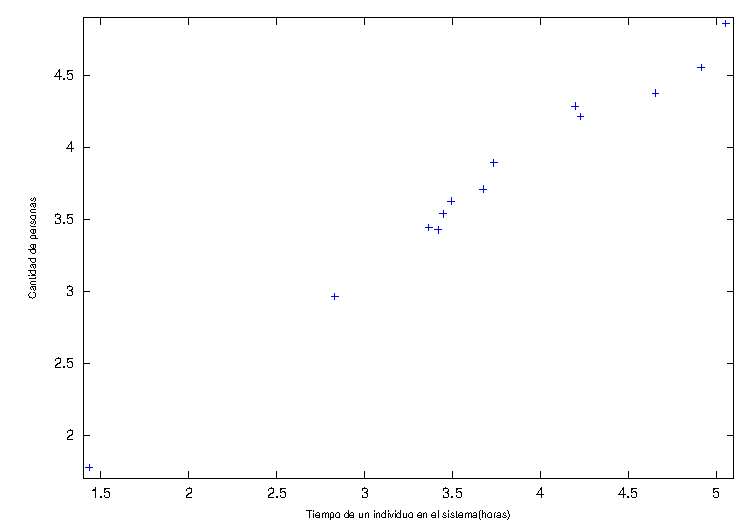
\includegraphics[scale=0.8]{graficos/LvsW}
\caption{Valor medio de individuos en el sistema  vs. Tiempo de un individuo en el sistema}
\label{fig:LvsW}
\end{figure*}

En la figura ~\ref{fig:mu} se observa que el tiempo medio de un individuo,
tanto en la cola como en el sistema, se incrementa a medida que aumenta el tiempo
medio que toma al servicio atender al cliente.
Para este gr\'{a}fico se toman $18$ valores distintos del par\'{a}metro $\mu$ y se
estudia su impacto en el tiempo medio de un individuo tanto en la cola
como en el sistema. Se realiza un an\'{a}lisis similar en la figura ~\ref{fig:tmediolambda},
esta vez con distintos valores del par\'{a}metro $\lambda$.


Es factible suponer que se incurre en determinados costos al mantener al
sistema en estado operativo. Los mismos pueden separarse en el costo
asociado a un cliente que espera, sea $c\frac{\$}{hora\ cliente}$, y el costo
propio de utilizaci\'{o}n del servidor, $s\frac{\$}{hora}$.


A partir de estas definiciones es posible computar el costo total medio, dado 
por:

\begin{equation}
\label{costo_total_medio}
C = \frac{1}{T} \int_{0}^{T} c(t) dt
\end{equation}

donde $c(t)$ es el costo total y $T$ es el tiempo de operaci\'{o}n.

En las figuras ~\ref{fig:ctmm} y ~\ref{fig:ctml} se presenta la evoluci\'{o}n
del costo total medio
al variar los par\'{a}metros $\mu$ y $\lambda$ respectivamente.


\section{Conclusiones}\label{conclusiones}

En un sistema de cola simple la estabilidad depende exclusivamente de la
intensidad de tr\'{a}fico. Se observa que peque\~{n}as variaciones en la tasa
de arribos o el tiempo medio de servicio pueden implicar grandes costos 
asociados.


Contar con informaci\'{o}n precisa de la cantidad de clientes a atender y la
frecuencia de llegada permite poder refinar la forma en que se presta el servicio,
buscando minimizar el tiempo de espera de los clientes y tambi\'{e}n el tiempo
en que cada servidor se encuentra inactivo.


\begin{figure*}[hp]
\centering
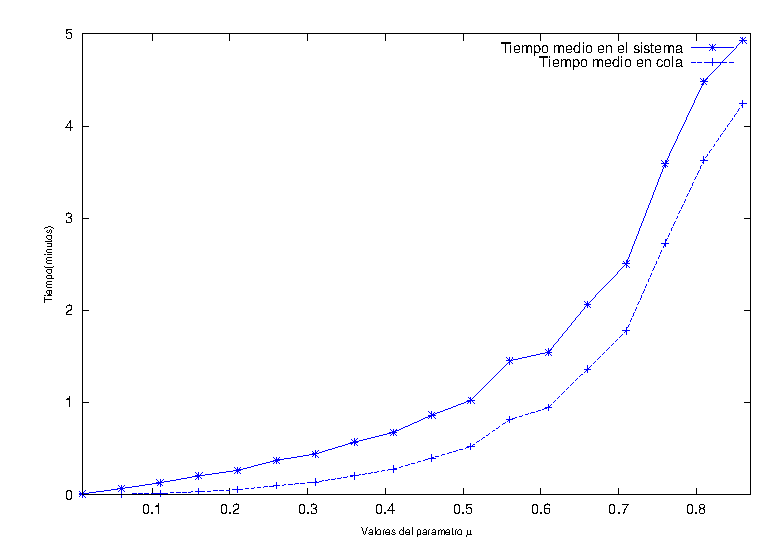
\includegraphics[scale=0.8]{graficos/tMediomu}
\caption{Tiempo medio vs. $\mu$}
\label{fig:mu}
\end{figure*}



\begin{figure*}[hp]
\centering
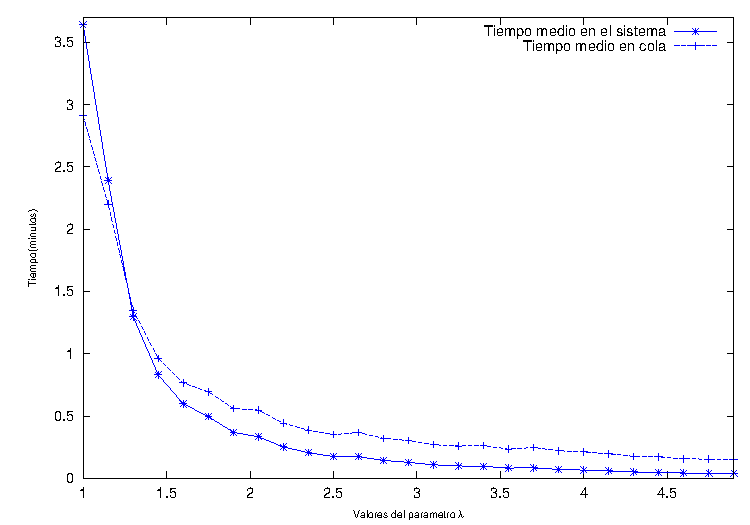
\includegraphics[scale=0.8]{graficos/tMedio}
\caption{Tiempo medio vs. $\lambda$}
\label{fig:tmediolambda}
\end{figure*}

\begin{figure*}[hp]
\centering
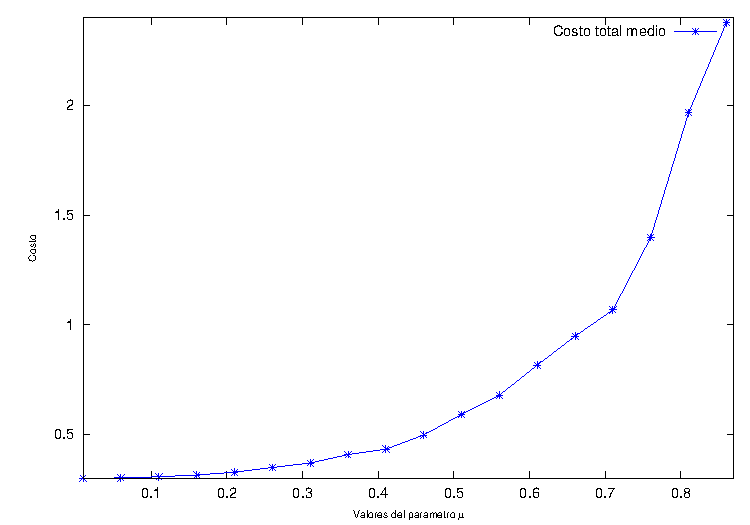
\includegraphics[scale=0.8]{graficos/CTMediomu}
\caption{Costo total medio vs. $\mu$}
\label{fig:ctmm}
\end{figure*}

\begin{figure*}[hp]
\centering
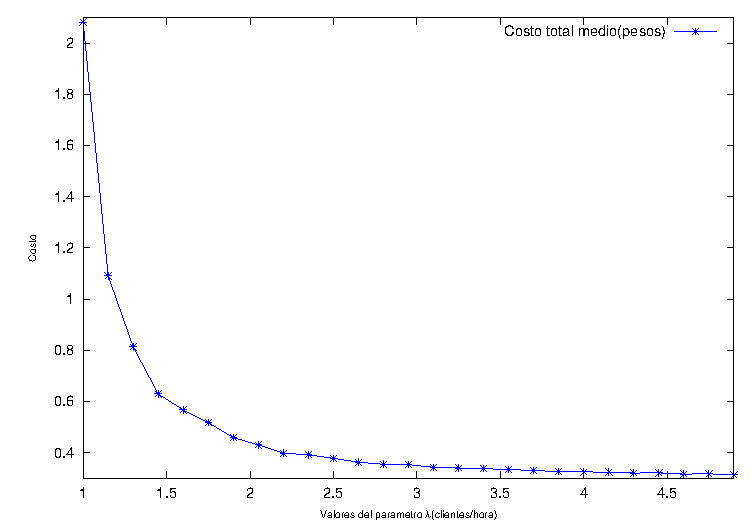
\includegraphics[scale=0.8]{graficos/CTMediolambda}
\caption{Costo total medio vs. $\lambda$}
\label{fig:ctml}
\end{figure*}



\end{document}
